\section{Results}
    \subsection{Initial Data Exploration}
    	See figures \ref{fig:language-frequency-plot} - \ref{fig:number-of-commits-1000-plot}
	    \begin{figure}
	        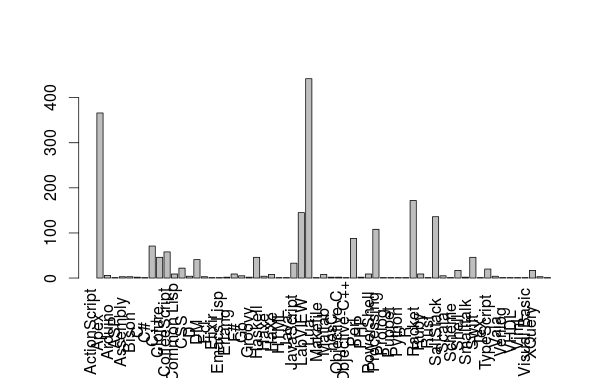
\includegraphics[width=250pt]{figures/language-frequency}
	        \caption{A histogram of the languages used in the projects}
	        \label{fig:language-frequency-plot}
	    \end{figure}

	    
	    \begin{figure}
	        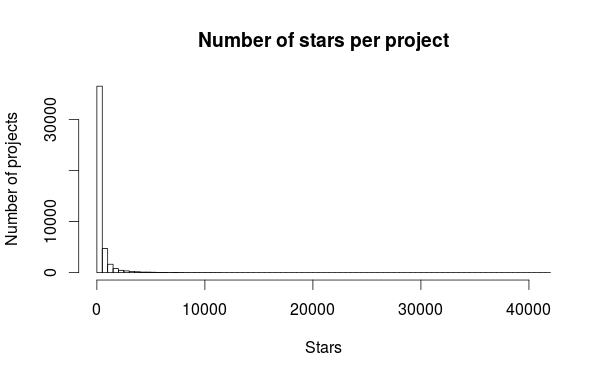
\includegraphics[width=250pt]{figures/star-distribution}
	        \caption{A histogram of the  number of stars per project}
	        \label{fig:star-distribution-plot}
	    \end{figure}
	    
	    \begin{figure}
	        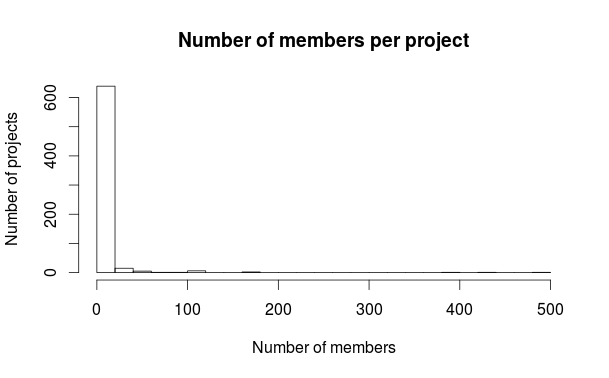
\includegraphics[width=250pt]{figures/number-of-members-per-project}
	        \caption{A histogram of the number of members per project}
	        \label{fig:number-of-members-per-project-plot}
	    \end{figure}
	    \begin{figure}
	        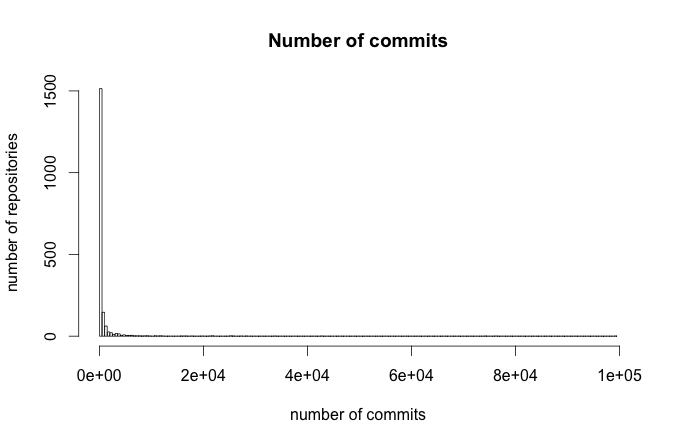
\includegraphics[width=250pt]{figures/number-of-commits-all}
	        \caption{A histogram of the number of commits per project}
	        \label{fig:number-of-commits-all-plot}
	    \end{figure}
	    \begin{figure}
	        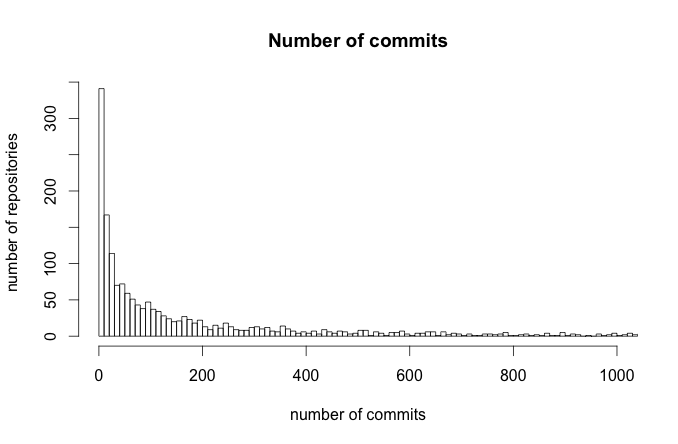
\includegraphics[width=250pt]{figures/number-of-commits-1000}
	        \caption{A histogram of the number of commits per project (with a maximum of 1000 commits)}
	        \label{fig:number-of-commits-1000-plot}

	    \end{figure}
    
    \subsection{Testing the model}
        \todo{Will be added later on, same for threats to validation}
